\documentclass[11pt,a4paper]{article}

% These are extra packages that you might need for writing the equations:
\usepackage{amsmath}
\usepackage{amsfonts}
\usepackage{amssymb}
\usepackage{booktabs}
\usepackage{hyperref}
\usepackage{listings}
\usepackage{xcolor}
\lstset {language=C++,
		 basicstyle=\ttfamily,
         keywordstyle=\color{blue}\ttfamily,
         stringstyle=\color{red}\ttfamily,
         commentstyle=\color{purple}\ttfamily,
         morecomment=[l][\color{magenta}]{\#},
       	 basicstyle=\tiny}

% You need the following package in order to include figures in your report:
\usepackage{graphicx}

% With this package you can set the size of the margins manually:
\usepackage[left=2cm,right=2cm,top=2cm,bottom=2cm]{geometry}


\begin{document}

% Enter the exercise number, your name and date here:
\noindent\parbox{\linewidth}{
 \parbox{.25\linewidth}{ \large ICP, Exercise 05 }\hfill
 \parbox{.5\linewidth}{\begin{center} \large Beat Hubmann \end{center}}\hfill
 \parbox{.2\linewidth}{\begin{flushright} \large Oct 28, 2018 \end{flushright}}
}
\noindent\rule{\linewidth}{2pt}


\section{Introduction}

To measure the fractal dimension of the percolating cluster in a square site lattice, both the Sandbox Algorithm and the Box Counting algorithm as described in~\cite{herrmann} were implemented. The largerst cluster found by the Hoshen-Kopelman algorithm~\cite{hoshen} was used as percolating cluster.

\section{Algorithm Description}
The Hoshen-Kopelman algorithm implementation was taken over from the previously submitted exercise 03.\\
Both the Sandbox and the Box Counting algorithm were implemented as described in the course lecture notes~\cite{herrmann}.\\
For the box counting method, the choice was made to double the cell size at each step until reaching the lattice size $L$, i.e. $\epsilon \in \{1, 2, 4, 8, \ldots, L\}$.

\section{Results}


The program was implemented as described above and submitted with this report. 
A square site lattice of side length $L=1024$ and occupation probabilities $p \in \{0.58, p_c=0.592746, 0.61\}$ were used.
As in the previous exercise, \texttt{C++}'s Mersenne Twister \texttt{mt19937} was used to initialize the lattices.

\subsection{Experiment 1: Sandbox Algorithm}
The box masses $M(R)$ where $M$ equals the numbers of sites occcupied by the largest (i.e. percolating) cluster at occupation probability $p$ in a box of increasing side length $R$ on a site lattice with side length $L=1024$, were recorded for $R \in \{3, 4, \cdots, L\}$. The results were plotted as $\log(M(R))$ versus $\log(R)$ as shown in figure~\ref{fig:1}.


\begin{figure}[ht]
\begin{center}
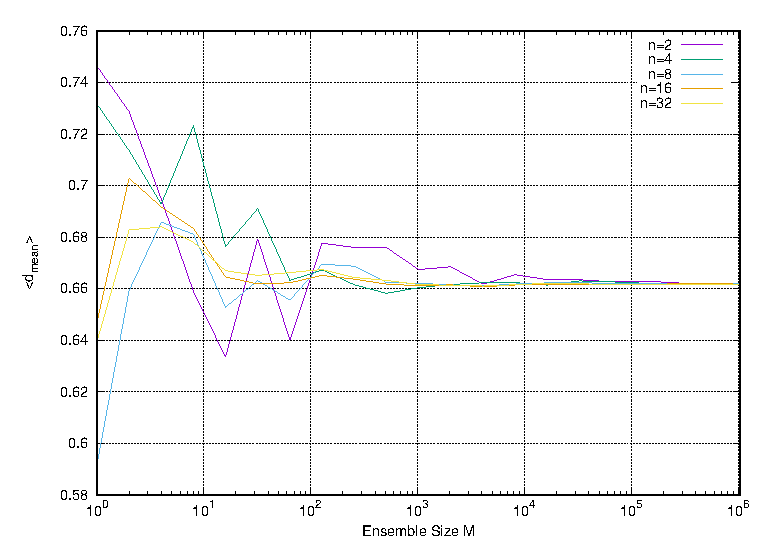
\includegraphics[scale=0.9]{figure1.eps} 
\end{center}
\caption{Sandbox Algorithm Results for $p \in \{0.58, p_c, 0.61\}$.}
\label{fig:1}
\end{figure}


\subsection{Experiment 2: Box Counting Algorithm}
The number of non-empty grid cells $N(\epsilon)$ where $\epsilon$ is the grid constant were recorded for $L=1024$ and $\epsilon \in \{1, 2, 4, 8, \ldots, L\}$ as described above. The results were plotted as $\log(N(\epsilon))$ versus $\log(\frac{1}{\epsilon})$ as shown in figure~\ref{fig:2}.



\begin{figure}[ht]
\begin{center}
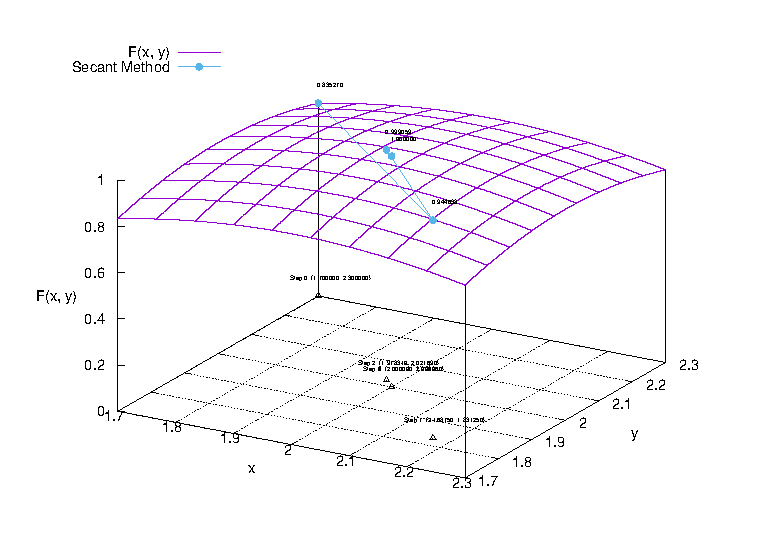
\includegraphics[scale=0.9]{figure2.eps} 
\end{center}
\caption{Box Counting Algorithm Results for $p \in \{0.58, p_c, 0.61\}$.}
\label{fig:2}
\end{figure}

\section{Discussion}
The slope of 1.88 of the line for $p=p_c$ in figure~\ref{fig:1} obtained from the Sandbox algorithm is well in line with the theoretical value of $d_f=\frac{91}{48} \approx 1.89$ for a 2D lattice and thus as expected.
For some reason reason, \texttt{gnuplot} couldn't be brought to fit a slope to the line for $p=p_c$ in figure~\ref{fig:2} obtained from the Box Counting algorithm. However, a visual inspection reveals that the slope is just a tad under 2 and thus in line with both the sandbox algorithm results and theoretical expectations. 

\begin{thebibliography}{99}

\bibitem{herrmann}
	Herrmann, H. J.,
	Singer, H. M.,
	Mueller L.,
	Buchmann, M.-A.,\\
	\emph{Introduction to Computational Physics - Lecture Notes},\\
	ETH Zurich,\\
	2017.
	
\bibitem{hoshen}
	Hoshen, J.,
	Kopelman, R.,\\
	\emph{Percolation and cluster distribution. I. Cluster multiple labeling technique and critical concentration algorithm},\\
	Phys. Rev. B 14, 3428,\\
	1976.

\end{thebibliography}


\end{document}